%% LaTeX-Beamer template for KIT design
%% by Erik Burger, Christian Hammer
%% title picture by Klaus Krogmann
%%
%% version 2.1
%%
%% mostly compatible to KIT corporate design v2.0
%% http://intranet.kit.edu/gestaltungsrichtlinien.php
%%
%% Problems, bugs and comments to
%% burger@kit.edu

\documentclass[18pt]{beamer}
%% SLIDE FORMAT
\usepackage[utf8]{inputenc}
\usepackage{enumitem}
% use 'beamerthemekit' for standard 4:3 ratio
% for widescreen slides (16:9), use 'beamerthemekitwide'

%\usepackage{templates/beamerthemekit}
\usepackage{wrapfig}
\usepackage{hyperref}
\usepackage{algpseudocode}
 \newcommand{\real}{\mathbb{R}}
 \newcommand{\nat}{\mathbb{N}}
 \newcommand{\Oh}{\mathcal{O}}
 \newcommand{\oh}{\mathrm{o}}
 \newcommand{\SP}{\mathrm{SP}}

% \usepackage{templates/beamerthemekitwide}

%\usepackage{epigraph}

% for quotes

\AtBeginSection[] % Do nothing for \section*
{
\begin{frame}<beamer>
\frametitle{Gliederung}
\tableofcontents[currentsection]
\end{frame}
}


\usepackage{biolinum}



%% TikZ INTEGRATION

% use these packages for PCM symbols and UML classes
% \usepackage{templates/tikzkit}
% \usepackage{templates/tikzuml}

% the presentation starts here

\title[Algo I Tut]{3. Algorithmen Tutorium I}
\subtitle{Datenstrukturen}
\author[Zangerle]{Konstantin Zangerle}

\institute{Institut für Theoretische Informatik}

\usepackage{listings}
\usepackage{color}

\definecolor{mygreen}{rgb}{0,0.6,0}
\definecolor{mygray}{rgb}{0.5,0.5,0.5}
\definecolor{mymauve}{rgb}{0.58,0,0.82}

\lstset{ %
  backgroundcolor=\color{white},   % choose the background color
  basicstyle=\footnotesize,        % size of fonts used for the code
  breaklines=true,                 % automatic line breaking only at whitespace
  captionpos=b,                    % sets the caption-position to bottom
  commentstyle=\color{mygreen},    % comment style
  escapeinside={\%*}{*)},          % if you want to add LaTeX within your code
  keywordstyle=\color{blue},       % keyword style
  stringstyle=\color{mymauve},     % string literal style
}

% Bibliography

\begin{document}

% change the following line to "ngerman" for German style date and logos
%\selectlanguage{ngerman}

%title page
\begin{frame}
\titlepage
\end{frame}

%table of contents
\begin{frame}{Gliederung}
 \tableofcontents
\end{frame}

\section{Besprechung der Übungsaufgaben}
\begin{frame}{Besprechung der Übungsaufgaben}
Häufige Fehler
\begin{itemize}
 \item ?
\end{itemize}

\end{frame}

\section{sqrt und log}
\begin{frame}{sqrt und log}
Einfacher als gedacht: \pause
 \begin{itemize}
  \item Beh: Es gilt: $\log \in \Oh(sqrt)$
  \item Bew: $\frac{\log(n)}{\sqrt(n)} = ?$ \pause
  \item Benutze L' Hospital:
  \item $dx \log x = \frac{1}{x}$
  \item $dx \sqrt x = \frac{1}{2} x^\frac{-1}{2}$
  \item $\lim_{x \to \infty} \frac{\log(n)}{\sqrt(n)} = \lim_{x \to \infty} \frac{1}{2 x^\frac{3}{2}} = 0$
 \end{itemize}

\end{frame}

\section{Datenstrukturen}

\begin{frame}{Eine Datenstruktur für...}
 Entwickle eine Datenstruktur, die folgende Eigenschaften hat:
 \begin{itemize}
  \item pushBack und popBack in $\Oh(1)$ im Worst-Case nicht nur amortisiert.
  \item Zugriff auf das k-te Element in $\Oh(log n)$ im Worst-Case nicht nur amortisiert.
 \end{itemize}
Eine Speicherallokation beliebiger Größe soll in $\Oh(1)$ funktionieren.
\end{frame}

\begin{frame}{Eine Datenstruktur für...}
 Entwickle eine Datenstruktur, die folgende Eigenschaften hat:
 \begin{itemize}
  \item pushBack und popBack in $\Oh(\log n)$ im Worst-Case nicht nur amortisiert.
  \item Zugriff auf das k-te Element in $\Oh(1)$ im Worst-Case nicht nur amortisiert.
 \end{itemize}
Eine Speicherallokation beliebiger Größe soll in $\Oh(1)$ funktionieren.
\end{frame}

\begin{frame}{Master Theorem}
 Zeigen Sie mit Hilfe des Master-Theorems scharfe asymptotische Schranken für folgende Rekurrenzen:
 
 \begin{enumerate}[label=\alph* )]
  \item $A(1) := 1$ und für $n = 2^k, k \in \mathbb{N}, A(n) = \sqrt{2} A(n/2) + \hat{c}^2 n$
  \item $B(1) := 4$ und für $n = 4^k, k \in \mathbb{N}, B(n) = 4B(n/4) + 4n$
  \item $C(1) := 3$ und für $n = 2^k, k \in \mathbb{N}, C(n) = 8C(n/2) + n$
  \item $D(1) := 2$ und für $n = 5^k, k \in \mathbb{N}, D(n) = 3(D(n/5)+2n + 1) + 3$
 \end{enumerate}

\end{frame}

\begin{frame}{Arrays}
 Gegeben sei ein Array $A = A[1], \ldots, A[n]$ mit n Zahlen in beliebiger Reihenfolge.
 Für eine gegebene Zahl x soll ein Paar $(A[i], A[j]), 1 \leq i, j \leq n$ gefunden werden,
 für gilt: $A[i] + A[j] = x$.
 
 \begin{enumerate}[label=\alph*)]
  \item Geben Sie eine Lösung für x = 33, und A = (7,15,21,14,18,3,9) an.
  \item Geben Sie einen effizienten Algorithmus an, der das Problem in erwarteter Zeit $\Oh(n)$
  löst, und bei Erfolg ein Paar (A[i], A[j]) ausgibt, ansonsten NIL.
 \end{enumerate}

\end{frame}


\begin{frame}
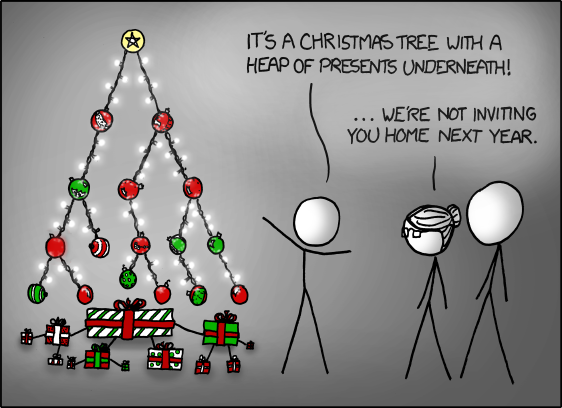
\includegraphics[scale=0.5]{tree} \\
License: http://creativecommons.org/licenses/by-nc/2.5/ \\
by xkcd.com/835
\end{frame}


\end{document}
